\documentclass[12pt]{article}
\usepackage{geometry}                % See geometry.pdf to learn the layout options. There are lots.
\geometry{letterpaper}                   % ... or a4paper or a5paper or ... 
%\geometry{landscape}                % Activate for for rotated page geometry
\usepackage[parfill]{parskip}    % Activate to begin paragraphs with an empty line rather than an indent
\usepackage{daves,fancyhdr,natbib,graphicx,dcolumn,amsmath,lastpage,url}
\usepackage{amsmath,amssymb,epstopdf,longtable}
\usepackage{paralist} 
\DeclareGraphicsRule{.tif}{png}{.png}{`convert #1 `dirname #1`/`basename #1 .tif`.png}
\pagestyle{fancy}
\lhead{CE 3372 -- Water Systems Design}
\rhead{SPRING 2025}
\lfoot{ES-14}
\cfoot{}
\rfoot{Page \thepage\ of \pageref{LastPage}}
\renewcommand\headrulewidth{0pt}



\begin{document}
\begin{center}
{\textbf{{CE 3372 -- Water Systems Design} \\ {Exercise Set 14}}}
\end{center}

\textbf{Purpose:}
Demonstrate application of SWMM for analysis of a detention pond as a stormwater control strategy.

\textbf{Objectives:}
\begin{itemize}
\item Compute depth and discharge in a detention pond using SWMM
\item Introduction to use of professional software (SWMM)
\item Develop expertise in interpreting output to answer specific hydraulic questions
\end{itemize}

\section*{\small{Exercise}}
Figure \ref{fig:detention} is a plan view of a rectangular detention pond.   

\begin{figure}[h!] %  figure placement: here, top, bottom, or page
   \centering
   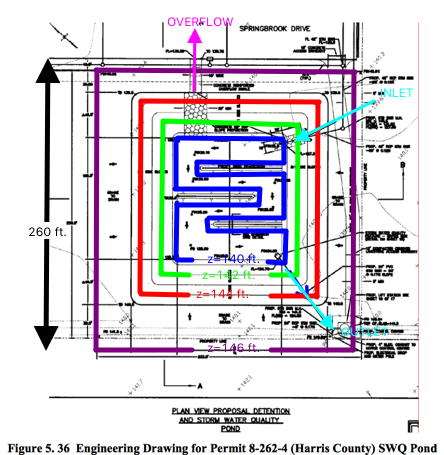
\includegraphics[width=4in]{detention.jpg} 
   \caption{Harris County, 8-262-4, Storm Water Quality Pond.}
   \label{fig:detention}
\end{figure}
\clearpage
The bottom of the pond is at elevation 139 feet.   
Several rectangular contour lines are shown.   
If the pond has one foot of water in storage, the blue line represents the pool elevation, and the volume would be the product of the area enclosed by the blue contour and the depth (1 foot).   
At depths greater than one foot, the pond sides are sloped and not vertical.

The inlet is a 1-foot diameter culvert that drains a 9-acre light-industrial complex.   
The invert elevation of this culvert at the pond is 139 feet.

The outlet works is a riser pipe which activates when the stage in the pond is 141 feet.
The diameter of the outlet pipe is 8-inches.
A secondary outlet pipe, also 8-inches activates at elevation 145 feet.

A small 4-inch drain pipe is at the pond bottom so that the pond drains completely after a storm.

If the pond stage exceeds 146 feet, the emergency overflow is a rectangular swale 25 feet wide and 2 feet deep which drains directly into a nearby bayou.

\begin{enumerate}
\item Figure \ref{fig:side-view} is a profile (elevation view of the pond).  Create your own sketch and label the inlet pipe, outlet pipe(s), and overflow swale; indicate the elevations of the pond bottom, inlet pipe invert (bottom) and soffit (top), the outlet pipe(s) invert(s) and soffit(s), and the invert elevation of the emergency overflow structure.
\begin{figure}[h!] %  figure placement: here, top, bottom, or page
   \centering
   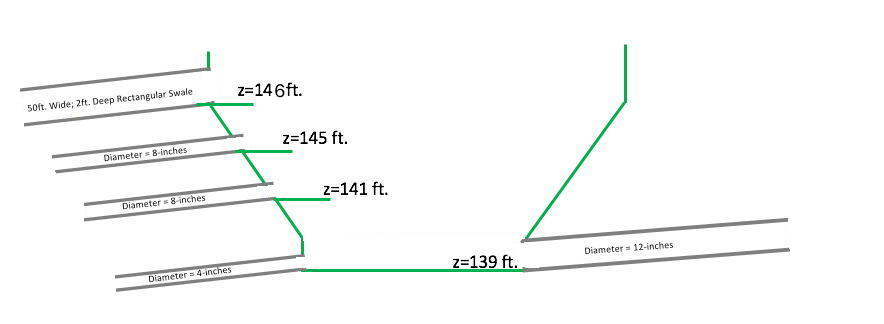
\includegraphics[width=6in]{side-view.jpg} 
   \caption{Schematic elevation-view sketch of pond.}
   \label{fig:side-view}
\end{figure}
\item Determine from Figure \ref{fig:detention} the depth-area relationships for pond stages of 0,1,2,3,4,5,6, 7 and 8 feet.   For the 8 foot stage, you can assume vertical walls extending upward from the z=146 feet contour line.   Prepare a table that lists water pool elevation, and water surface area.  
\item Build a SWMM model of the detention pond (Storage Node; Tabular Depth-Area).   
The catchment that drains to the pond can be modeled as a 9-acre square region, with an overland slope of 0.05\%.
Use an appropriate value for runoff coefficient.   
The inlet pipe is a 1-foot diameter, 200-foot long RCP, laid on a slope of 0.05\%.
The outlet pipes and overflow swale are also at slope 0.05\%; they are also 200 feet long.

The multiple outlets will need to connect to a common junction node 200 feet from the pond, which will then connect to an outfall.  The connection to the outfall should be a 6-foot diameter conduit, 200 feet long.   Set the outfall as a \texttt{FREE} outfall boundary condition.
\item Run the SWMM model using a constant intensity of 3-inches per hour for 6 hours.  Prepare output plots of pond depth versus time, pond inflow versus time, and pond outflow versus time.

Determine:
\begin{enumerate}[a)]
\item If the pond overflows with this particular rainfall input?
\item The maximum constant-intensity, 6-hour storm that the pond can accommodate without activating the overflow spillway.
\item The pond's effective (without activating the overflow spillway) annual recurrence interval (ARI) given that the time of concentration for the contributing area is 15 minutes.  
\end{enumerate}


\end{enumerate}



\end{document}  